% Template LaTeX file for DAFx-19 papers
%
% To generate the correct references using BibTeX, run
%     latex, bibtex, latex, latex
% modified...
% - from DAFx-00 to DAFx-02 by Florian Keiler, 2002-07-08
% - from DAFx-02 to DAFx-03 by Gianpaolo Evangelista
% - from DAFx-05 to DAFx-06 by Vincent Verfaille, 2006-02-05
% - from DAFx-06 to DAFx-07 by Vincent Verfaille, 2007-01-05
%                          and Sylvain Marchand, 2007-01-31
% - from DAFx-07 to DAFx-08 by Henri Penttinen, 2007-12-12
%                          and Jyri Pakarinen 2008-01-28
% - from DAFx-08 to DAFx-09 by Giorgio Prandi, Fabio Antonacci 2008-10-03
% - from DAFx-09 to DAFx-10 by Hannes Pomberger 2010-02-01
% - from DAFx-10 to DAFx-12 by Jez Wells 2011
% - from DAFx-12 to DAFx-14 by Sascha Disch 2013
% - from DAFx-15 to DAFx-16 by Pavel Rajmic 2015
% - from DAFx-16 to DAFx-17 by Brian Hamilton 2016
% - from DAFx-18 to DAFx-19 by Dave Moffat 2019
%
% Template with hyper-references (links) active after conversion to pdf
% (with the distiller) or if compiled with pdflatex.
%
% 20060205: added package 'hypcap' to correct hyperlinks to figures and tables
%                      use of \papertitle and \paperauthorA, etc for same title in PDF and Metadata
% 05/02/2019: Package 'hypcap' removed, and replaced with 'caption', to allow for the inclusion
%			of a CC UP licence.
%
% 1) Please compile using latex or pdflatex.
% 2) If using pdflatex, you need your figures in a file format other than eps! e.g. png or jpg is working
% 3) Please use "paperftitle" and "pdfauthor" definitions below

%------------------------------------------------------------------------------------------
%  !  !  !  !  !  !  !  !  !  !  !  ! user defined variables  !  !  !  !  !  !  !  !  !  !  !  !  !  !
% Please use these commands to define title and author(s) of the paper:
\def\papertitle{REAL-TIME IMPLEMENTATION OF AN ELASTO-PLASTIC FRICTION MODEL APPLIED TO STIFF STRINGS USING FINITE-DIFFERENCE SCHEMES}
\def\paperauthorA{Silvin Willemsen}
\def\paperauthorB{Stefania Serafin}
\def\paperauthorC{Stefan Bilbao}

% Authors' affiliations have to be set below

%------------------------------------------------------------------------------------------
\documentclass[twoside,a4paper,dvipsnames]{article}
\usepackage{tikz}
\tikzset{>=latex}
\tikzstyle{block} = [draw,minimum size=0.5cm]
\usetikzlibrary{math,arrows,positioning,shapes.geometric, decorations.markings}
% \tikzset{MyArrow/.style={single arrow, draw, minimum width=1mm, minimum height=10mm,
%                          inner sep=0mm, single arrow head extend=1mm}
% }
\usepackage{dafx_19}
\usepackage{amsmath,amssymb,amsfonts,amsthm}
\usepackage{euscript}
\usepackage[latin1]{inputenc}
\usepackage[T1]{fontenc}
\usepackage{ifpdf}
\usepackage{scalerel}
\usepackage[]{algorithm2e, setspace}
\usepackage{multicol}
\newcommand\norm[1]{\left\lVert#1\right\rVert}
\usepackage[english]{babel}
\usepackage{caption}
\usepackage{subfig} % or can use subcaption package
\usepackage{color}
\usepackage{diagbox}
\usepackage{multirow}
\newenvironment{rcases}
  {\left.\begin{alignedat}{2}}
  {\end{alignedat}\right\rbrace}
\DeclareMathOperator{\sgn}{sgn}
\setcounter{page}{1}
\ninept

\usepackage{times}
% Saves a lot of ouptut space in PDF... after conversion with the distiller
% Delete if you cannot get PS fonts working on your system.

% pdf-tex settings: detect automatically if run by latex or pdflatex
\newif\ifpdf
\ifx\pdfoutput\relax
\else
   \ifcase\pdfoutput
      \pdffalse
   \else
      \pdftrue
\fi

\ifpdf % compiling with pdflatex
  \usepackage[pdftex,
    pdftitle={\papertitle},
    pdfauthor={\paperauthorA, \paperauthorB},
    colorlinks=false, % links are activated as colror boxes instead of color text
    bookmarksnumbered, % use section numbers with bookmarks
    pdfstartview=XYZ % start with zoom=100% instead of full screen; especially useful if working with a big screen :-)
  ]{hyperref}
  \pdfcompresslevel=9
%   \usepackage[pdftex]{graphicx}
%  \usepackage[figure,table,hypcap=true]{caption}
\else % compiling with latex
  
  \usepackage[dvips]{epsfig,graphicx}
  \usepackage[dvips,
    colorlinks=false, % no color links
    bookmarksnumbered, % use section numbers with bookmarks
    pdfstartview=XYZ % start with zoom=100% instead of full screen
  ]{hyperref}
  % hyperrefs are active in the pdf file after conversion
%  \usepackage[figure,table,hypcap=true]{caption}
\fi
  \usepackage[hypcap=true]{caption}
\title{\papertitle}

%-------------SINGLE-AUTHOR HEADER STARTS (uncomment below if your paper has a single author)-----------------------
%\affiliation{
%\paperauthorA \,\sthanks{This work was supported by the XYZ Foundation}}
%{\href{http://dafx2019.bcu.ac.uk/}{Digital Media Technology Lab} \\ Birmingham City University \\ Birmingham, UK \\ {\tt \href{mailto:dafx2019@gmail.com}{dafx2019@gmail.com}}}
%-----------------------------------SINGLE-AUTHOR HEADER ENDS------------------------------------------------------

%---------------TWO-AUTHOR HEADER STARTS (uncomment below if your paper has two authors)-----------------------
\threeaffiliations{
\paperauthorA}
{{Multisensory Experience Lab, CREATE,} \\ Aalborg University Copenhagen\\
  Copenhagen, Denmark\\ {\tt \href{mailto:sil@create.aau.dk}{sil@create.aau.dk}}}
{\paperauthorC}
{ Acoustics and Audio Group \\ University of Edinburgh\\
    Edinburgh, UK\\
     {\tt \href{mailto:s.bilbao@ed.ac.uk}{s.bilbao@ed.ac.uk}}}
     {\paperauthorB}
{{Multisensory Experience Lab, CREATE,} \\ Aalborg University Copenhagen\\
  Copenhagen, Denmark\\ {\tt \href{mailto:sts@create.aau.dk}{sts@create.aau.dk}}}
%-------------------------------------TWO-AUTHOR HEADER ENDS------------------------------------------------------

%---------------THREE-AUTHOR HEADER STARTS (uncomment below if your paper has three authors)-----------------------
% \threeaffiliations{
% \paperauthorA \,\sthanks{This work was supported by the XYZ Foundation}}
% {\href{http://dafx2019.bcu.ac.uk/}{Digital Media Technology Lab} \\ Birmingham City University \\ Birmingham, UK \\ {\tt \href{mailto:dafx2019@gmail.com}{dafx2019@gmail.com}}}
% {\paperauthorB \,\sthanks{Thanks to the predecessors for the templates}}
% {\href{http://dafx2018.web.ua.pt/}{IEETA} \\ University of Aveiro \\ Aveiro, Portugal \\ {\tt \href{mailto:dafx2018_papers@ua.pt}{dafx2018\_papers@ua.pt}}}
% {\paperauthorC \,\sthanks{Illustrious contributor}}
% {\href{http://www.acoustics.ed.ac.uk}{Acoustics and Audio Group,} \\ University of Edinburgh\\ Edinburgh, UK\\ {\tt \href{mailto:dafx17@ed.ac.uk}{dafx17@ed.ac.uk}}}
%-------------------------------------THREE-AUTHOR HEADER ENDS------------------------------------------------------

%----------------FOUR-AUTHOR HEADER STARTS (uncomment below if your paper has four authors)-----------------------
% \fouraffiliations{
% \paperauthorA \,\sthanks{This work was supported by the XYZ Foundation}}
% {\href{http://dafx2019.bcu.ac.uk/}{Digital Media Technology Lab} \\ Birmingham City University \\ Birmingham, UK \\ {\tt \href{mailto:dafx2019@gmail.com}{dafx2019@gmail.com}}}
% {\paperauthorB \,\sthanks{Thanks to the predecessors for the templates}}
% {\href{http://dafx2018.web.ua.pt/}{IEETA} \\ University of Aveiro \\ Aveiro, Portugal \\ {\tt \href{mailto:dafx2018_papers@ua.pt}{dafx2018\_papers@ua.pt}}}
% {\paperauthorC \,\sthanks{Illustrious contributor}}
% {\href{http://www.acoustics.ed.ac.uk}{Acoustics and Audio Group,} \\ University of Edinburgh\\ Edinburgh, UK\\ {\tt \href{mailto:dafx17@ed.ac.uk}{dafx17@ed.ac.uk}}}
% {\paperauthorD \,\sthanks{This guy is a very good fellow}}
% {\href{http://dafx16.vutbr.cz}{SPLab} \\ Brno University of Technology \\ Brno, Czech Republic \\ {\tt \href{mailto:dafx16@vutbr.cz}{dafx16@vutbr.cz}}}
%-------------------------------------FOUR-AUTHOR HEADER ENDS------------------------------------------------------

\usepackage{xcolor}
\def\SBcomment[#1]{\textcolor{Red}{#1}}
\def\SWcomment[#1]{\textcolor{Green}{#1}}

\begin{document}
% more pdf-tex settings:
\ifpdf % used graphic file format for pdflatex
  \DeclareGraphicsExtensions{.png,.jpg,.pdf, .eps} 
\else  % used graphic file format for latex
  \DeclareGraphicsExtensions{.eps}
\fi

\maketitle
    
\begin{abstract}
The simulation of a bowed string is challenging due to the strongly non-linear relationship between the bow and the string. This relationship can be described through a model of friction. Several friction models in the literature have been proposed, from simple velocity dependent to more accurate ones. Similarly, a highly accurate technique to simulate a stiff string is the use of finite-difference time-domain (FDTD) methods. As these models are generally computationally heavy, implementation in real-time is challenging. This paper presents the combination of a complex friction model, namely the elasto-plastic friction model, and a stiff string simulated using FDTD methods. We show that it is possible to keep the CPU usage of a single bowed string below 5 percent. For real-time control of the bowed string, the Sensel Morph is used.
\end{abstract}
\section{Introduction}
\label{sec:intro}
In physical modelling sound synthesis applications, the simulation of a bowed string is a challenging endeavour. This is mainly due to the strongly non-linear relationship between the bow and the string, through a model of friction. Such friction models can be categorised as static or dynamic; models of the latter type have only recently seen a major effort. As opposed to static friction models, where friction depends only on the relative velocity of the two bodies in contact, dynamic models describe the friction force through a differential equation.

 A recently popular dynamic model is the elasto-plastic model, first proposed in \cite{Dupont2002}. The model assumes that the friction between the two objects in contact is caused by a large ensemble of bristles, each of which contributes to the total friction force. The average bristle deflection is used as an extra independent variable for calculating the friction force. As shown in \cite{Serafin2003}, the elasto-plastic model can be applied to a bowed string simulation and it exhibits a hysteresis loop in the force versus velocity plane due to this multivariable dependency.
 This is consistent with recent measurement performed using a bowing machine in \cite{Woodhouse2003}.
 The elasto-plastic model has been thoroughly investigated in a musical context by Serafin et al. in \cite{Serafin2003, Serafin2004, Avanzini2005}. 

Regarding bowed string simulations, the first musical non-linear systems, including bowed strings, were presented by McIntyre, et al. in \cite{McIntyre1983}. Smith published the first real-time implementation of the bowed string using a digital waveguide (DW) for the string and a look-up table for the friction model in \cite{Smith1986}. Simultaneously, Florens, et al. published a real-time implementation using mass-spring systems for the string and a static friction model for the bow in \cite{Florens1986}. 

The dynamics of musical instruments are generally described by systems of  partial differential equations (PDEs). Specialised synthesis methods such as DWs \cite{Smith1992} and modal synthesis \cite{Morrison1993} are derived from particular solutions.  Mainstream time-stepping methods such as finite-difference time-domain (FDTD) methods were first proposed in \cite{Hiller, Hiller2, Chaigne}, and developed subsequently \cite{Bilbao2009, Bilbao2018}. In \cite{Maestre2014} the authors adapted the thermal model proposed by Woodhouse \cite{Woodhouse2003} for real-time applications using a DW for the string implementation and a combination of the DW and FDTD methods for the bowing interaction. In \cite{Desvages2017, Desvages2015}, Desvages used FDTD methods for the implementation of the string in two polarizations and a static double exponential friction model introduced in \cite{Smith2000}. This was, however, not implemented in real-time. To the best of the authors' knowledge, the only known real-time implementation of any bow model applied to complete FDTD strings was presented in \cite{Willemsen2019} where the soft exponential friction function presented in \cite{Bilbao2009} was used. The current work can be considered an extension of this work.

We are interested in bridging the gap between highly accurate physical models and efficient implementations so that these models can be played in real-time. In this work, we present an implementation of the elasto-plastic friction model in conjunction with a finite-difference implementation of the damped stiff string. Furthermore, we show that it is possible to play the string in real-time using the Sensel Morph controller \cite{Sensel2019}.

This paper is structured as follows. In Section \ref{sec:elasto}, the elasto-plastic bow model in conjunction with a PDE model for a stiff string is described. Discretisation is covered in Section \ref{sec:discretisation}, and implementation details appear in Section \ref{sec:implementation}. In Section \ref{sec:results}, simulated results are presented and discussed. Some concluding remarks appear in Section  \ref{sec:conclusion}.

\section{Elasto-Plastic Bow Model}\label{sec:elasto}

Consider a linear model of transverse string vibration in a single polarization, where $u(x,t)$ represents string displacement as a function of time $t\geq 0$, in s, and coordinate $x\in[0,\,L]$ (in m) for some string length $L$ (in m). Using the subscripts $t$ and $x$ to denote differentiation with respect to time and space respectively, a partial differential equation describing the dynamics of the damped stiff string is \cite{Bilbao2009}
\begin{equation}\label{eq:PDE}
    u_{tt} = c^2u_{xx}-\kappa^2u_{xxxx}-2\sigma_0u_t+2\sigma_1u_{txx}.
\end{equation}
Here $c = \sqrt{T/\rho A}$ is the wave speed (in m/s) with tension $T$ (in N), material density $\rho$ (in kg$\cdot$m$^{-3}$) and cross-sectional area $A$ (in m$^2$). Furthermore, $\kappa = \sqrt{EI/\rho A}$ is the stiffness coefficient (in m$^2$/s) with Young's Modulus $E$ (in Pa), area moment of inertia $I$ (in m$^4$). For a string of circular cross section we have radius $r$, cross-sectional area $A=\pi r^2$ and area moment of inertia $I=\pi r^4 /4$.  Lastly, $\sigma_0 \geq 0$ (in s$^{-1}$) and $\sigma_1 \geq 0$ (in m$^2$/s) 
%\SWcomment[these units for the damping coefs are correct, right?] 
are coefficients allowing for frequency-independent and frequency-dependent damping respectively. 

In our implementation we assume simply supported boundary conditions, which are defined as
\begin{equation}
    u = u_{xx} = 0 \quad \text{where} \quad x = 0, L\, .
\end{equation}
% \SWcomment[No curly brackets for $x = \{0,L\}$? Is that because you can't have sets in the continuous domain?]

\begin{figure}[h]
    \centering
    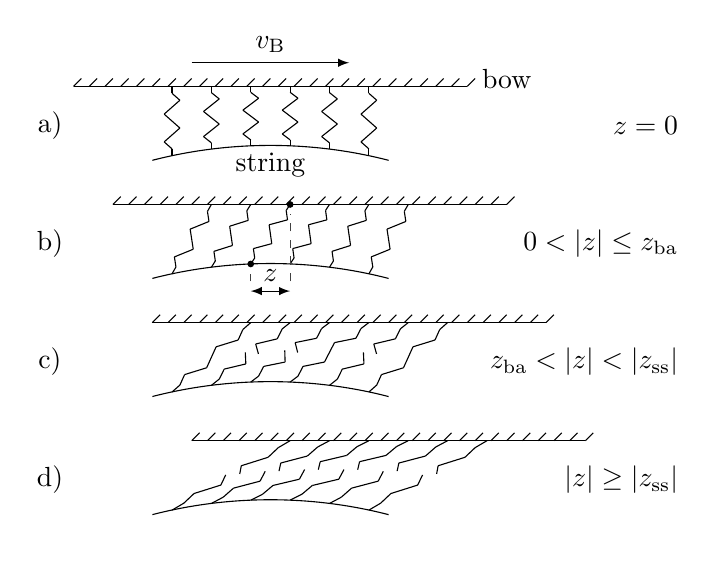
\begin{tikzpicture}
    
    \def\radius{6}; % Radius of the string (>2!)
    \pgfmathsetmacro{\reps}{3}; % How may back-and-forths in the drawing of the springs
    \def\horShift{0.5}; %how far the bow is shifted to the right in b)
    \def\bowSpacing{0.2};
    \def\drawingSpacing{1.5}
    \def\bowWidth{5};
    
    %subfigure letters
    \node (A) at (-2.8, 0.5) {a)};
    \node (B) at (-2.8, 0.5 - \drawingSpacing) {b)};
    \node (C) at (-2.8, 0.5 - \drawingSpacing * 2) {c)};
    \node (D) at (-2.8, 0.5 - \drawingSpacing * 3) {d)};
    
    %bow velocity arrow
    \draw[->] (-1, 1.3) -- (1, 1.3) node [midway, above] (velText) {$v_\text{B}$};
    
    \pgfmathsetmacro{\zCoordTop}{0};
    \pgfmathsetmacro{\zYCoordBottom}{0};
    \def\springForZ{2}
    \foreach \drawing in {0, ..., 3}
    {
        %% Draw String
        \begin{scope}
            \clip (-1.5,-0.2- \drawing * \drawingSpacing) rectangle (1.5,1.5);
            \draw (0,-\radius + 0.25 - \drawing * \drawingSpacing) circle(\radius);
        \end{scope}

        %% Draw Bow
        \def\halfBW{\bowWidth*0.5}
        \pgfmathsetmacro{\halfNumDiag}{0.5 * \bowWidth / \bowSpacing};
        \draw[-] (-\halfBW + \drawing * \horShift,1 - \drawing * \drawingSpacing) -- (\halfBW + \drawing * \horShift, 1 - \drawing * \drawingSpacing);
        \foreach \bowDiag in {-\halfNumDiag, ...,\halfNumDiag}
        {
        \pgfmathtruncatemacro{\bD}{\bowDiag}
        % \ifnum\drawing=0
        %     \ifnum\bD<-1
        %         \draw[-] (\drawing * \horShift + \bowDiag * \bowSpacing, -\drawing * \drawingSpacing + 1) -- (\drawing * \horShift + \bowDiag * \bowSpacing + 0.1, -\drawing * \drawingSpacing + 0.1 + 1);
        %         \else
        %         \ifnum\bD>1
        %             \draw[-] (\drawing * \horShift + \bowDiag * \bowSpacing, -\drawing * \drawingSpacing + 1) -- (\drawing * \horShift + \bowDiag * \bowSpacing + 0.1, \drawing * -2 + 0.1 + 1);
        %         \fi
        %     \fi
        % \else
            \draw[-] (\drawing * \horShift + \bowDiag * \bowSpacing, -\drawing * \drawingSpacing + 1) -- (\drawing * \horShift + \bowDiag * \bowSpacing + 0.1, -\drawing * \drawingSpacing + 0.1 + 1);
        % \fi
            
        }
        
        \def\brokenSprings{{0, 1, 1, 0, 1, 0}};
        %% Draw Springs
        \foreach \springNo in {0, ..., 5}
        {
            % Calculate spring length depending on the radius of the string
            \pgfmathsetmacro{\startX}{\springNo  * 0.5 - 1.25};
            \pgfmathsetmacro{\calcSpace}{(\radius + 1) - \radius * sin(acos(\startX/\radius)) - 0.25};
            \pgfmathsetmacro{\springLength}{sqrt(\calcSpace*\calcSpace+\drawing*\horShift*\drawing*\horShift)};
            
            \pgfmathsetmacro{\spacing}{\springLength / (\reps + 2)}; 
            % spacing between two spring-back-and-forths
            \ifnum\drawing=0
                \pgfmathsetmacro{\rot}{0};
            \else
                \pgfmathsetmacro{\rot}{(270+(atan(\calcSpace/(\drawing*\horShift))))}; %rotation of the springs
            \fi
            
            \ifnum\drawing=1
                \ifnum\springNo=\springForZ
                    \pgfmathsetmacro{\resTwo}{sqrt(\springLength*\springLength-\horShift*\horShift)};
                    \global\let\zCoordBottom = \resTwo;
                \fi
            \fi
        
            \pgfmathsetmacro{\isBroken}{\brokenSprings[\springNo]};
            % debug code
            % \node (nodeTest\springNo) at (\springNo*1.1-2, -3 - 1 * \drawing + 0.3 * \springNo) {\isBroken};
            
            \begin{scope}[shift={(\startX + \drawing * \horShift,1 -\drawing * \drawingSpacing)}]
                \pgfmathsetmacro{\xWidth}{0.1 - (\drawing * 0.02)};
                \draw[-, rotate = \rot] (0, 0) -- (0, -\spacing * 0.5);
                \draw[-, rotate = \rot] (0, -\spacing * 0.5) -- (\xWidth, -\spacing);
                \def\Y{-\spacing}
                \foreach \idx in {1,...,\reps}
                {
                    \pgfmathsetmacro{\idxMinOne}{\idx-1};
                    \ifnum\drawing=2
                        \ifnum\isBroken=1
                            \pgfmathtruncatemacro{\idxT}{\reps * 0.5 + 1}
                            \ifnum\idx=\idxT
                                \draw[-, rotate = \rot] (\xWidth, \Y - \idxMinOne * \spacing) -- (-\xWidth,\Y - \idx * \spacing*0.6);
                                \draw[-, rotate = \rot] (\xWidth, \Y - \idxMinOne * \spacing * 1.66) -- (-\xWidth,\Y - \idx * \spacing);
                            \else
                                \draw[-, rotate = \rot] (\xWidth, \Y - \idxMinOne * \spacing) -- (-\xWidth,\Y - \idx * \spacing);
                            \fi
                        \else
                                \draw[-, rotate = \rot] (\xWidth, \Y - \idxMinOne * \spacing) -- (-\xWidth,\Y - \idx * \spacing);
                        \fi
                    \else
                        \ifnum\drawing=3
                            \pgfmathtruncatemacro{\idxT}{\reps * 0.5 + 1}
                            \ifnum\idx=\idxT
                                \draw[-, rotate = \rot] (\xWidth, \Y - \idxMinOne * \spacing) -- (-\xWidth,\Y - \idx * \spacing*0.6);
                                \draw[-, rotate = \rot] (\xWidth, \Y - \idxMinOne * \spacing * 1.66) -- (-\xWidth,\Y - \idx * \spacing);
                            \else
                                \draw[-, rotate = \rot] (\xWidth, \Y - \idxMinOne * \spacing) -- (-\xWidth,\Y - \idx * \spacing);
                            \fi
                        \else
                            \draw[-, rotate = \rot] (\xWidth, \Y - \idxMinOne * \spacing) -- (-\xWidth,\Y - \idx * \spacing);
                        \fi
                    \fi
                    \pgfmathsetmacro{\invXWidth}{\xWidth*-1};
                    \global\let\xWidth = \invXWidth;
                    \pgfmathsetmacro{\lastYPre}{\Y - \idx * \spacing};
                    \global\let\lastY = \lastYPre;
                }
                \draw[-, rotate = \rot] (\xWidth, \lastY) -- (0, \lastY - \spacing * 0.5);
                \draw[-, rotate = \rot] (0, \lastY - \spacing * 0.5) -- (0, \lastY - \spacing);
             \end{scope}
             
        }
        % \draw[<->] (2,2-0.707) -- node[right] {$r=\sqrt{2} \Rightarrow A=\pi(\sqrt{2})^2=2\pi$} (2,2+0.707);
        
        % \node(stringText) at (0, -\drawing * 2) {string};
        % \node[block, minimum height = 0.15cm, fill=white, draw=white] (bowText) at (\drawing * \horShift, 1.23 - \drawing * 2) {bow};
    }
    \filldraw[black] (-1.25+\springForZ*0.5 + \horShift,1-\drawingSpacing) circle (1pt) node[anchor=center](topZ){};
    \filldraw[black] (-1.25++\springForZ*0.5,1-\zCoordBottom-\drawingSpacing) circle (1pt) node[anchor=center](bottomZ){};
    
    \node [](leftNode) at (-1.25+\springForZ*0.5,-\drawingSpacing - 0.1) {};
    \node [](rightNode) at (-1.25 +\springForZ*0.5 + \horShift,-\drawingSpacing - 0.1) {};
    
    \draw[<->] (leftNode.center) -- (rightNode.center) node [midway, above] (TextNode) {$z$};
    \draw[dashed, darkgray] (leftNode) -- (bottomZ);
    \draw[dashed, darkgray] (rightNode) -- (topZ);
    %% Draw bow and string texts
        \node(stringText) at (0, 0) {string};
        \node(bowText) at (3, 1.1) {bow};
    %% Draw descriptions of z
    \def\zTexts{{"$z=0$", "$0<|z|<z_{\text{ba}}$", "$z_{\text{ba}}<|z|< z_\text{ss}$", "$|z|>z_\text{ss}$"}};
    
    \node[anchor = east](zText1) at (5.3, 0.5) {$z=0$};
    \node[anchor = east](zText1) at (5.3, 0.5 - \drawingSpacing) {$0<|z|\leq z_{\text{ba}}$};
    \node[anchor = east](zText1) at (5.3, 0.5 - \drawingSpacing * 2) {$z_{\text{ba}}<|z|< |z_\text{ss}|$};
    \node[anchor = east](zText1) at (5.3, 0.5 - \drawingSpacing * 3) {$|z|\geq|z_\text{ss}|$};
    
    \end{tikzpicture}
    \caption{\it Microscopic displacements of the bristles between the bow and the string. The bow moves right with a velocity of $v_\text{B}$. a) The initial state is where the average bristle displacement $z=0$. b) The bow has moved right relative to the string. The purely elastic, or presliding regime is entered (stick). c) After the break-away displacement $z_\text{ba}$, more and more bristles start to `break'. This is defined as the elasto-plastic regime. d) After all bristles have `broken', the steady state (slip) is reached and the purely plastic regime is entered.}
    \label{fig:elastoPlastic}
\end{figure}

As mentioned in the introduction, the elasto-plastic bow model assumes that the friction between the bow and the string is due to a large ensemble of bristles, each of which contributes to the total friction force. See Figure \ref{fig:elastoPlastic} for a graphical representation of this. The bristles are assumed to be damped stiff springs and can `break' after a given break-away displacement threshold. An extra term can be added to \eqref{eq:PDE} to include the bowing interaction
\begin{equation}
    \begin{aligned}
    \label{eq:bowingTerm}
        u_{tt} = \hdots - \delta(x-x_\text{B})f(v, z)/\rho A.
    \end{aligned}
\end{equation}
Here, the spatial Dirac delta function $\delta(x-x_\text{B})$ allows for the pointwise application of the force $f$ at externally supplied bowing position $x_\text{B}(t)$. 

%The force $f$ is dependent on the relative velocity $v$ between the string at the bowing point and the bow itself, %defined as
 In the following we will use the definitions found in \cite{Dupont2002}. The force $f$ is defined in terms of the relative velocity $v$ and average bristle displacement $z$ (see Figure \ref{fig:elastoPlastic}) as
\begin{equation}\label{eq:forceFunction}
    f(v, z) = s_0z + s_1\dot z + s_2v + s_3w,
\end{equation}
where \begin{equation}\label{eq:relVel}
  v = u_t(x_\text{B}) - v_\text{B},
\end{equation}
where $v_\text{B}(t)$ is an externally supplied bow velocity,
$s_0$ is the bristle stiffness (in N/m), $s_1$ is the damping coefficient (in kg/s), $s_2$ is the viscous friction (in kg/s) and $s_3$ is a dimensionless noise coefficient multiplied onto pseudorandom function $w(t)$ (in N) as done in \cite{Serafin2004} and adds noise to the friction force. Here, $\dot{z}$ indicates a time derivative of $z$, and is related to $v$ through
\begin{equation}\label{eq:zdot}
    \dot z = r(v, z) = v \bigg[ 1-  \alpha(v, z)\frac{z}{z_\text{ss}(v)}\bigg],
\end{equation}
where $z_\text{ss}$ is the steady-state function
\begin{equation}\label{eq:zss}
    z_\text{ss}(v) = \frac{\sgn(v)}{s_0}\Big[f_\text{C}+(f_\text{S}-f_\text{C})e^{-(v/v_\text{S})^2}\Big],
\end{equation}
with Stribeck velocity $v_\text{S}$ (in m/s), Coulomb force $f_\text{C} = f_\text{N}\mu_\text{C}$ and stiction force $f_\text{S} = f_\text{N}\mu_\text{S}$ (both in N). Here $\mu_\text{C}$ and $\mu_\text{S}$ are the dynamic and static friction coefficient respectively and $f_\text{N}(t)$ is the normal force (in N) which is, like $v_\text{B}(t)$, externally supplied. See Figure \ref{fig:zss} for a plot of \eqref{eq:zss}. 

\begin{figure}[ht]
\centerline{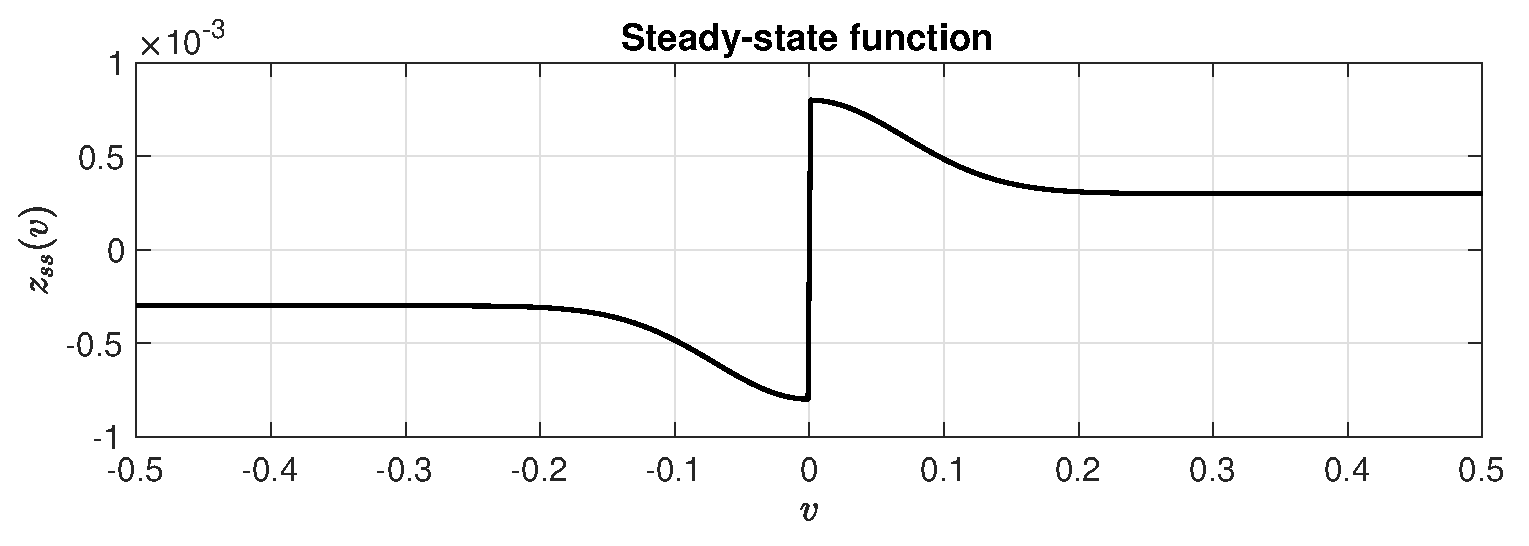
\includegraphics[width=1.0\columnwidth]{steadyState.eps}}
\caption{\label{fig:zss}{\it A plot of the steady-state function $z_\text{ss}(v)$ with a force of 10 N.}}
\end{figure}
Furthermore, the adhesion map between the bow and the string is defined as
\begin{equation}\label{eq:adhesionMap}
\alpha(v, z) = 
\begin{aligned}
    \begin{cases}
    \begin{rcases}
        &0 & |z| \leq z_\text{ba}\\
       &\alpha_\text{m}(v,z)&\ \, z_\text{ba}<|z|<|z_\text{ss}(v)|\\        &1 &|z|\geq|z_\text{ss}(v)|
        \end{rcases} 
        
        &\!\!\!\!\!\text{if}\  \sgn(v)=\sgn(z)\\
        \,0&\!\!\!\!\!\text{if}\  \sgn(v)\neq\sgn(z),
    \end{cases}
    \end{aligned}
\end{equation}
where the transition between the elastic and plastic behaviour is defined as
\begin{equation}\label{eq:alphaM}
    \alpha_\text{m} = \frac{1}{2}\bigg[1+\sgn(z)\sin\bigg(\pi\frac{z-\sgn(z)\frac{1}{2}(|z_\text{ss}(v)|+z_\text{ba})}{|z_\text{ss}(v)|-z_\text{ba}}\bigg)\bigg],
\end{equation}
with break-away displacement $z_\text{ba}$, i.e., where the bristles start to break (see Figure \ref{fig:elastoPlastic} c)). A plot of the adhesion map can be found in Figure \ref{fig:alphaPlot}.\footnote{It is interesting to note is that in the literature on this topic such as \cite{Dupont2002, Serafin2003, Serafin2004, Avanzini2005}, a few inaccuracies can be found in the definition of $\alpha(v,z)$: 1) all uses of $z_\text{ss}$ in \eqref{eq:adhesionMap} and \eqref{eq:alphaM} lack the absolute value operator, 2) the multiplications with $\sgn(z)$ in \eqref{eq:alphaM} are excluded, 3) $\alpha(v,z)$ is undefined for $|z|=z_\text{ba}$ and $|z|=|z_\text{ss}(v)|$ (correct in the original paper by Dupont et al. \cite{Dupont2002}). It can be shown that only with the definitions presented here, is it possible to obtain the curve shown in Figure \ref{fig:alphaPlot}.}

One of the difficulties in working with this model is that, due to the many approximations, the notion of an energy balance, relating the rate of stored energy in the system to power input and loss is not readily available. Such energy methods are used frequently in the context of physical modeling synthesis and virtual analog modeling as a means of arriving at numerical stability conditions for strongly nonlinear systems, as is the present case. See, e.g., \cite{Bilbao2009}. This means that we do not have a means of ensuring numerical stability in the algorithm development that follows. This does not mean, however, that an energy balance is not available. 

\begin{figure}[ht]
\centerline{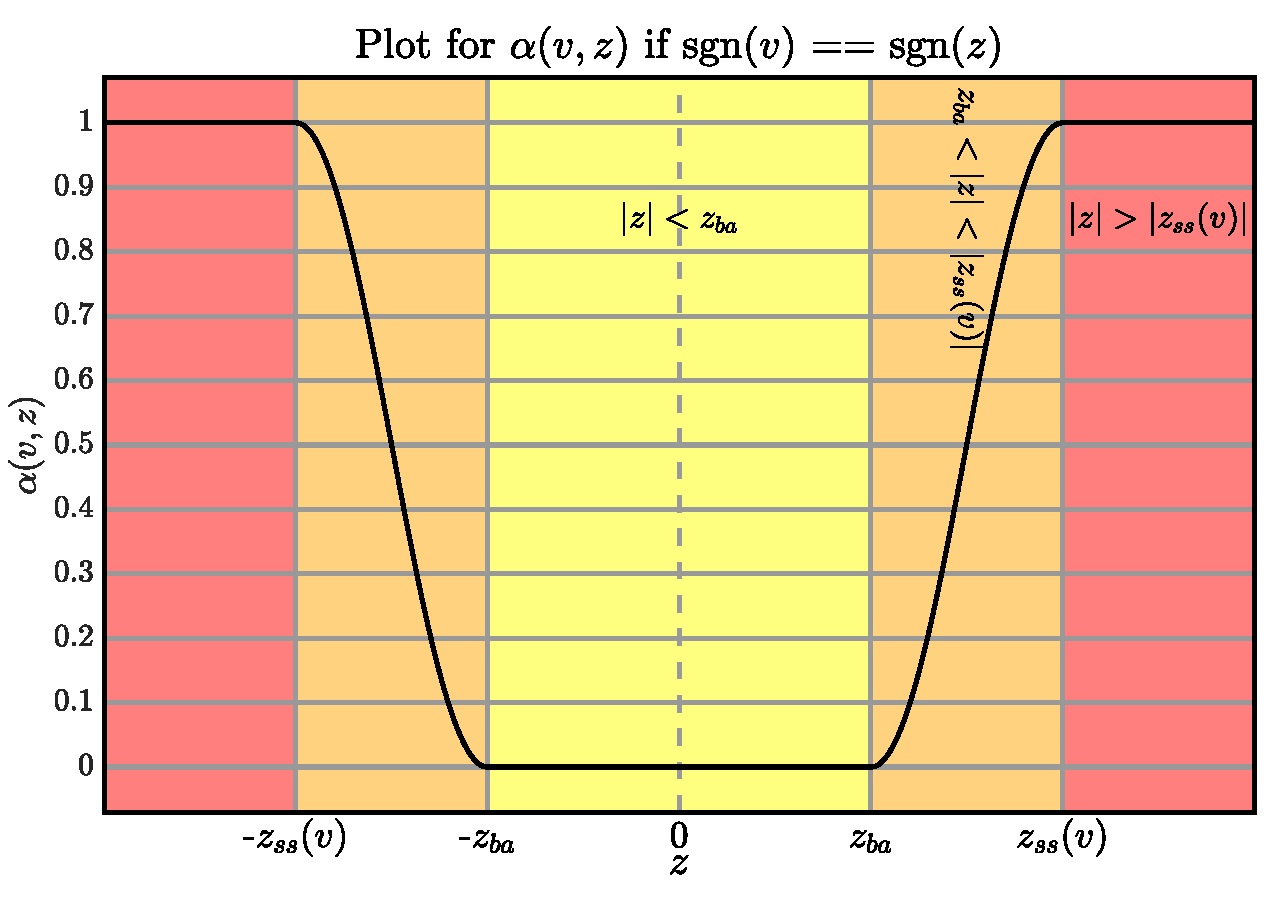
\includegraphics[width=1.0\columnwidth]{drawAlpha.eps}}
\caption{\label{fig:alphaPlot}{\it A plot of the adhesion map $\alpha(v,z)$ plotted against $z$ when the signs of $v$ and $z$ are the same. The different regions of the map are shown with the coloured areas and correspond to Figure \ref{fig:elastoPlastic} according to: yellow - a) \& b), orange - c) and red - d).}}
\end{figure}

\section{Discretisation}\label{sec:discretisation}
Finite-difference schemes for the stiff string in isolation are covered by various authors \cite{Chaigne, Bilbao2009}. 

Equation \eqref{eq:PDE} can be discretised at times $t = nk$, with sample $n \in \mathbb{N}$ and time-step $k = 1 / f_\text{s}$ with sample-rate $f_\text{s}$ and locations $x = lh$, where grid spacing $h$ needs to abide the following condition \cite{Bilbao2009}
\begin{equation}\label{eq:stability}
    h \geq h_\text{min} = \sqrt{\frac{c^2k^2+4 \sigma_1k+\sqrt{(c^2k^2+4\sigma_1k)^2+16\kappa^2k^2}}{2}}
\end{equation}
and grid points $l \in [0,...,N]$, where $N=\text{floor}(L/h)$ and $N + 1$ is the total number of grid points. It is important to note that the closer $h$ is to $h_\text{min}$, the more accurate the scheme will be. 
Approximations for the derivatives found in \eqref{eq:PDE} are described in the following way \cite{Bilbao2009}: 
\begin{subequations}\label{eq:approximations}
    \begin{align}
        % \label{eq:secondSpacey}\delta_{yy}u_l^n &= \frac{1}{h^2}\big(u_{m+1}^n - 2u_m^n + u_{m-1}^n\big),\\
        %  \label{eq:fourthSpace}\delta_xxxx &= \frac{1}{h^4}\big(u_{l+2}^n - 4u_{l+1}^2 + 6 u_{l}^n - 4u_{l-1}^n + u_{l-2}^n\big),\\
        \label{eq:centerTime}
        u_{t} &\approx \delta_{t\cdot} u^n_l = \frac{1}{2k}\big(u_l^{n+1}-u_l^{n-1}\big),\\
        \label{eq:secondTime}
        u_{tt} &\approx \delta_{tt}u_l^n = \frac{1}{k^2} \big(u_l^{n+1} - 2u_l^n + u_l^{n-1}\big),\\
        \label{eq:secondSpacex}
        u_{xx} &\approx \delta_{xx}u_l^n = \frac{1}{h^2}\big(u_{l+1}^n - 2u_l^n + u_{l-1}^n\big),\\
        u_{txx} &\approx \label{eq:timeSpace}
        \begin{aligned}[t]\delta_{t-}\delta_{xx}u_l^n =& \; \frac{1}{hk^2}\big(u_{l+1}^n - 2u_l^n + u_{l-1}^n \\
        &- u_{l+1}^{n-1} + 2u_l^{n-1} - u_{l-1}^{n-1}\big),
        \end{aligned}\\
        \label{eq:fourthSpacex}
        u_{xxxx} &\approx\begin{aligned}[t] \delta_{xxxx}u_l^n = \frac{1}{h^4}\big(&u_{l+2}^n - 4u_{l+1}^n + 6u_l^n \\
        &- 4u_{l-1}^n +u_{l-2}^n\big),
        \end{aligned}
    \end{align}
\end{subequations}
with grid function $u_l^n$ denoting a discretised version of $u(x,t)$ at the $n$th time step and the $l$th point on the string. Note that in \eqref{eq:timeSpace}, the backwards time difference operator is used to keep \eqref{eq:FDS} explicit and thus computationally cheaper to update. Using the approximations shown in \eqref{eq:approximations}, \eqref{eq:bowingTerm} can be discretised to
\begin{equation}
  \begin{aligned}
    \label{eq:FDS}
        \delta_{tt} u_l^n = &\: c^2 \delta_{xx} u_l^n -\kappa^2\delta_{xxxx} u_l^n - 2\sigma_0\delta_{t\cdot} u_l^n
        \\ 
        &+ 2\sigma_1\delta_{t-}\delta_{xx}u_l^n - J(x_\text{B}^n)f(v^n, z^n) / \rho A,
    \end{aligned}
\end{equation}
where the relative velocity described in \eqref{eq:relVel} can be discretised as
\begin{equation}\label{eq:discRelVel}
v^n = I(x_\text{B}^n)\delta_{t\cdot}u_l^n -  v_\text{B}^n.
\end{equation}
    Here, $I(x_\text{B}^n)$ and $J(x_\text{B}^n)$ are weighting functions where the former interpolates the string displacement and velocity and the latter distributes the bowing term around time-varying bowing position $x_\text{B}^n$ (see Figure \ref{fig:interpol} and \cite{Bilbao2009}
for more details on this). Furthermore,
\begin{equation}\label{eq:discForceFunction}
    f(v^n,z^n) = s_0z^n + s_1r^n+s_2v^n+s_3w^n
\end{equation} 
is the discrete counterpart of \eqref{eq:forceFunction} where 
\begin{equation}\label{eq:r}
    r^n = r(v^n,z^n) = v^n\bigg[1-\alpha(v^n,z^n)\frac{z^n}{z_\text{ss}(v^n)}\bigg]
\end{equation}
is the discrete counterpart of \eqref{eq:zdot}.
\begin{figure}[h]
    \centering
    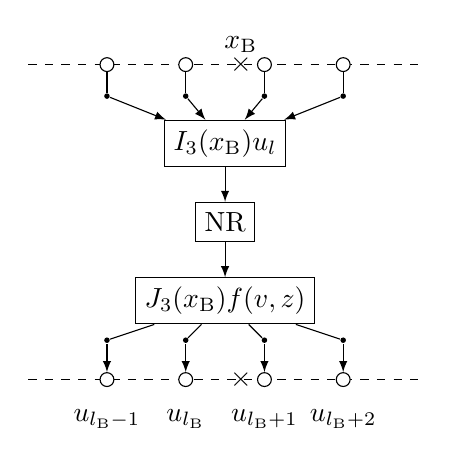
\begin{tikzpicture}
    %  \draw [->] (0 0) edge (1 1);
    \draw[dashed] (0, 0) -- (5, 0);
     \node [block, draw=black](J) at (2.5, 1) {$J_3(x_\text{B})f(v,z)$};
     \node (u1) at (1, -0.5) {$u_{l_\text{B}-1}$};
     \node (u2) at (2, -0.5) {$u_{l_\text{B}}$};
     \node (u3) at (3, -0.5) {$u_{l_\text{B}+1}$};
     \node (u4) at (4, -0.5) {$u_{l_\text{B}+2}$};
     
    \foreach \id in {1,...,4}
    {
        \node [circle, draw=black, fill=white, inner sep=0pt,minimum size=5pt](a\id) at (\id, 0) {};
        \node [circle, fill=black, inner sep=0pt,minimum size=2pt](b\id) at (\id, 0.5) {};
        \draw [<-] (a\id) -- (b\id);
        \draw [-] (b\id) edge (J);
    }
    \node [block](NR) at (2.5, 2) {NR};
    \node [block](I) at (2.5, 3){$I_3(x_\text{B})u_l$};
    \draw[dashed] (0, 4) -- (5, 4);
    \foreach \id in {1,...,4}
    {
        \node [circle, draw=black, fill=white, inner sep=0pt,minimum size=5pt](c\id) at (\id, 4) {};
        \node [circle, fill=black, inner sep=0pt,minimum size=2pt](d\id) at (\id, 3.6) {};
        \draw [-] (c\id) -- (d\id);
        \draw [->] (d\id) edge (I);
    }
    \node(x) at (2.7, 4) {$\times$};
    \node(x) at (2.7, 0) {$\times$};
    \node(xb) at (2.7, 4.25) {$x_\text{B}$};
    \draw [->] (I) edge (NR);
    \draw [->] (NR) edge (J);
    
\end{tikzpicture} 
    \caption{\it Cubic interpolation at bowing point $x_\text{B}$. The interpolator $I$ retrieves the values of four grid points which are then used in the Newton-Raphson (NR) solver. This outputs the force function $f(v,z)$ that the spreading function $J$ in turn distributes over the same four grid points. This process happens every single sample. %See Appendix \ref{app:interpol} for more details.
    }
    \label{fig:interpol}
\end{figure}

At the bowing point we need to iteratively solve for two unknown variables: the relative velocity between the bow and the string $v$ and the mean bristle displacement $z$ of the bow.
We can solve \eqref{eq:FDS} at $x_\text{B}^n$ using \eqref{eq:discRelVel} and identity \cite{Bilbao2009}
\begin{equation}
    \delta_{tt}u_l^n = \frac{2}{k}\big(\delta_{t\cdot}u_l^n-\delta_{t-}u_l^n\big)
\end{equation}
resulting in 
%\begin{equation}
%\label{eq:stiffStringFDS}
%\begin{aligned}
%\frac{2}{k}&\Big(v + v_\text{B}\Big) - \frac{2}{k^2}I(x_\text{B}^n)\delta_{t-}u_l^n  = \; c^2 I(x_\text{B}^n)\delta_{xx} u_l^n \\
%&-\kappa^2I(x_\text{B}^n)\delta_{xxxx} u_l^n - 2\sigma_0(v
%+ v_\text{B})\\
%&+ 2\sigma_1I(x_\text{B}^n)\delta_{t-}\delta_{xx}u_l^n - J(x_\text{B}^n)f(v, z).
%\end{aligned}
%\end{equation}
\begin{equation} \label{eq:incIdentity}
    I(x_\text{B}^n)J(x_\text{B}^n)f(v^n,z^n)/\rho A+\Big(\frac{2}{k}+2\sigma_{0}\Big) v^n+b^n = 0,
\end{equation}
% \SWcomment[or does this still need to be scaled by 1/h for it to be correctly solved in NR?]{}\SBcomment[Yes, you need the $1/h$...but (15) is only true if you use a pure spreading function selecting just one point...why not just do this? Otherwise you need to worry about the size of I*J. If you're moving the bow around, though, you definitely need this product though. ]
where 
\begin{equation}\label{eq:bn}
        \begin{aligned}b^n =& \: \frac{2}{k}v_\text{B}^n-\frac{2}{k}I(x_\text{B}^n)\delta_{t-}u_l^n - c^2 I(x_\text{B}^n)\delta_{xx} u_l^n +\kappa^2I(x_\text{B}^n)\delta_{xxxx} u_l^n \\
    &+ 2\sigma_0v_\text{B}^n -2\sigma_1I(x_\text{B}^n)\delta_{t-}\delta_{xx}u_l^n
\end{aligned}
\end{equation}
and can be pre-computed as its terms are not dependent on $v$ or $z$. Recalling \eqref{eq:forceFunction}, this can be rewritten to
\begin{equation}\label{eq:newtonFunction}
\begin{aligned}
    % J(x_\text{B}^n)\Big(
    &I(x_\text{B}^n)J(x_\text{B}^n)\Bigg(\frac{s_0z^n+s_1r^n+s_2v^n+s_3w^n}{\rho A}
    \Bigg)\\
    &+\Big(\frac{2}{k} + 2\sigma_0 \Big)v^n+ b^n= 0.
    \end{aligned}
\end{equation}
% \SWcomment[is it ok to interpret the spreading operator like this? Also, I could include the $s_3w$ in $b$ instead (as it is not dependent on $v$ or $z$) but then it would be confusing when using $J$ for spreading the force as $s_3w$ is also part of the force function in  \eqref{eq:forceFunction}.] \SBcomment[OK, I don't get why you need the spreading operator anymore...] \SWcomment[For the scaling by $1/h$, or don't I need this anymore here?] 
% \begin{equation}\label{eq:newtonFunction}
%     % J(x_\text{B}^n)\Big(
%     s_0z+s_1((\mu_{t+})^{-1}\delta_{t+}) z+(s_2 + (\frac{2}{k} + 2\sigma_0)\rho A)v+s_3w
%     % \Big)
%     + b\rho A = 0\end{equation}
% \SWcomment[This is how I am trying to implement it now: first multiplying everything in \eqref{eq:incIdentity} by $\rho A$ and then solving this for $v$ in \eqref{eq:velCalc}.]

% Moreover,
%     \begin{equation}
%         \begin{aligned}b =& \: \frac{2}{k}v_\text{B}-\frac{2}{k}I(x_\text{B}^n)\delta_{t-}u_l^n - c^2 I(x_\text{B}^n)\delta_{xx} u_l^n +\kappa^2I(x_\text{B}^n)\delta_{xxxx} u_l^n \\
%     &+ 2\sigma_0v_\text{B} -2\sigma_1I(x_\text{B}^n)\delta_{t-}\delta_{xx}u_l^n.
% \end{aligned}
% \end{equation}
% and can be pre-computed as its terms are not dependent on $v$ or $z$.

To obtain the values of $v^n$ and $z^n$, multivariate Newton-Raphson (NR) is used. If \eqref{eq:newtonFunction} is defined to be $g_1  = g_1(v^n, z^n)$ and 
\begin{equation}\label{eq:g2}
   g_2(v^n, z^n) = r^n - a^n = 0,
\end{equation}
with
\begin{equation}\label{eq:an}
    a^n = (\mu_{t-})^{-1}\delta_{t-} z^n
\end{equation}
(where the operators applied to $z^n$ denote the trapezoid rule \cite{Bilbao2009}) we obtain the following iteration 
\begin{equation}\label{eq:NRit}
    \begin{bmatrix}
    v_{(i+1)}^n\\
    z_{(i+1)}^n
    \end{bmatrix}
    =
    \begin{bmatrix}
    v_{(i)}^n\\
    z_{(i)}^n
    \end{bmatrix}
    -
    \begin{bmatrix}
    \frac{\partial g_1}{\partial v} & \frac{\partial g_1}{\partial z}\\
    \frac{\partial g_2}{\partial v} & \frac{\partial g_2}{\partial z}\\
    \end{bmatrix}^{-1}
    \begin{bmatrix}
    g_1\\
    g_2
    \end{bmatrix}\,
    ,
\end{equation}
where $i$ is the iteration number capped by 50 iterations, and the convergence threshold is set to $10^{-7}$.
% To obtain the values of $v$ and $z$ at sample $n$, an iterative solving method such as Newton-Raphson (NR) needs to be used and is defined as \cite{Wallis1685}
% \begin{equation}
%     y_{i+1} = y_{i} - \frac{g(y_i)}{g'(y_i)} \quad \text{while} \quad |y_{i+1}-y_i| > \phi
% \end{equation}
% where $g(y)$ is an arbitrary function dependent on to-be-calculated variable $y$ at iteration index $i$. The calculation is done until the difference between the unknown variable at the next iteration and the current iteration is smaller than a threshold $\phi$.

% As we need to find the roots of \eqref{eq:zdot}, $g$ with $y=\dot z$ is defined as
% \begin{equation}
%   g(\dot z) = v\bigg[1-\alpha(v, z)\frac{z}{z_\text{ss}(v)}\bigg] -  \dot z(v,z) = 0,
% \end{equation}
% and
% \begin{equation}
%     \dot z_{(i+1)} = \dot z_{(i)} - \frac{g(\dot z_{(i)})}{g'(\dot z_{(i)})}
% \end{equation}
% where
% \begin{equation}\label{eq:derivativeG}
%     g'(\dot z_{(i)}) = -\frac{s_1}{s_2+\frac{2}{k} + 2\sigma_0}\frac{\partial g(\dot z_{(i)})}{\partial v} + \frac{k}{2}\frac{\partial g(\dot z_{(i)})}{\partial z} - 1.
% \end{equation}
% % \begin{equation}\label{eq:derivativeG}
% %     g'(\dot z^i) = -\frac{s_1}{s_2+(\frac{2}{k} + 2\sigma_0)\rho A}\frac{dg(\dot z^i)}{dv} + \frac{k}{2}\frac{dg(\dot z^i)}{dz} - 1.
% % \end{equation}
% The derivatives in \eqref{eq:derivativeG} can be found in \cite{Serafin2004}. In the NR iteration, the newly calculated value for $\dot z$ and the values of $z$ and $\dot z$ at the previous time step are used to calculate an estimate of $z$ using the trapezoid rule
% \begin{equation}\label{eq:trapRule}
%     z^n = z^{n-1} + \frac{k}{2}(\dot z_{(i+1)} + \dot z^{n-1}).
% \end{equation}
% Inserting this into \eqref{eq:newtonFunction} we can calculate $v$ using
% \begin{equation}\label{eq:velCalc}
%     v = \frac{-s_0z-s_1\dot z-s_3w-b}{s_2 + \frac{2}{k} + 2\sigma_0}.
% \end{equation}
% % \begin{equation}\label{eq:velCalc}
% %     v = \frac{-s_0z-s_1\dot z-s_3w-b\rho A}{s_2 + (\frac{2}{k} + 2\sigma_0)\rho A}.
% % \end{equation}
% From \eqref{eq:trapRule} and \eqref{eq:velCalc} it is now also clear how the coefficients that the derivatives in \eqref{eq:derivativeG} are multiplied with are obtained. 

\section{Implementation}\label{sec:implementation}
In this section, we will elaborate on the implementation; the parameters used and the system architecture. The real-time implementation of the discrete-time model shown in the previous section has been done using C++ together with the JUCE framework \cite{JUCE}. The application is shown in Figure \ref{fig:application}. The parameters we used can be found in Table \ref{tab:parameters}, most of which are based on implementations by Serafin in \cite{Serafin2004}. These parameters will be static, i.e., are not user-controlled (except for $z_\text{ba}$ and $s_3$ which rely on $f_\text{N}$). A demonstrative video can be found in \cite{video}.
    
\begin{table}[ht]
  \caption{{\it Parameter values (with fundamental frequency $f_0$ and sample rate $f_\text{s}$).}}
	\centering
  \begin{tabular}{|c|c|c|c|}\hline
    Parameter & Symb. (unit) & Value (notes)\\ \hline
    Material Density &$\rho$ (kg$\cdot$m$^{-3}$) & $7850$ \\
    Radius & $r$ (m) & $5\cdot10^{-4}$\\
    String length & $L$ (m) & $1$\\
    Wave speed & $c$ (m/s) & $2 f_0/L$\\
    Young's modulus & $E$ (Pa) & $2\cdot 10^{11}$\\
    Freq. indep. damping & $\sigma_0$ (s$^{-1}$) & $1$\\
    Freq. dep. damping & $\sigma_1$ (m$^{2}$/s) & $5 \cdot 10^{-3}$\\
    Coulomb friction & $\mu_\text{C}$ (-) & $0.3$ ($<\mu_\text{S}$) \\
    Static friction & $\mu_\text{S}$ (-) & $0.8$ ($>\mu_\text{C}$) \\
    Normal force & $f_\text{N}$ (N) & 10 \\
    Bow velocity & $v_\text{B}$ (m/s) & 0.1 \\
    Bow position & $x_\text{B}$ (m) & 0.25 \\
    Stribeck velocity & $v_\text{S}$ (m/s) & $0.1$ \\
    Bristle stiffness & $s_0$ (N/m)& $10^4$ \\
    Bristle damping & $s_1$ (kg/s)& $0.001\sqrt{s_0}$ \\
    Viscous friction & $s_2$ (kg/s) & $0.4$ \\
    Noise coefficient & $s_3$ (-) & $0.05f_\text{N}$\\
    Pseudorandom func. & $w$ (N) & $-1<w<1$\\
    Break-away disp.& $z_\text{ba}$ (m) & $0.7 f_\text{C}/s_0$ ($<f_\text{C}/s_0$) \\
    Time step & $k$ (s) & $1/f_\text{s}$ \\
    %NR threshold & $\phi$ (-) & $10^{-7}$ \\
    \hline
 \end{tabular}
	%
  \label{tab:parameters}
\end{table}
We use the passivity condition proposed by \cite{Astrom2008} for our choices of different parameter-values. As this condition applies to the LuGre model first proposed in \cite{Canudas1993, Canudas1995} from which the elasto-plastic model evolved, further investigation is required to conclude whether these conditions are identical for the elasto-plastic model.
\subsection{Sensel Morph}
As mentioned in Section \ref{sec:intro}, the Sensel Morph (or Sensel for short) is used as an interface to control the bowed string (see Figure \ref{fig:sensel}). The Sensel is a highly sensitive touch controller containing ca. 20,000 pressure sensitive sensors that allow for expressive control of the implementation \cite{Sensel2019}.
\begin{figure}[ht]
\centerline{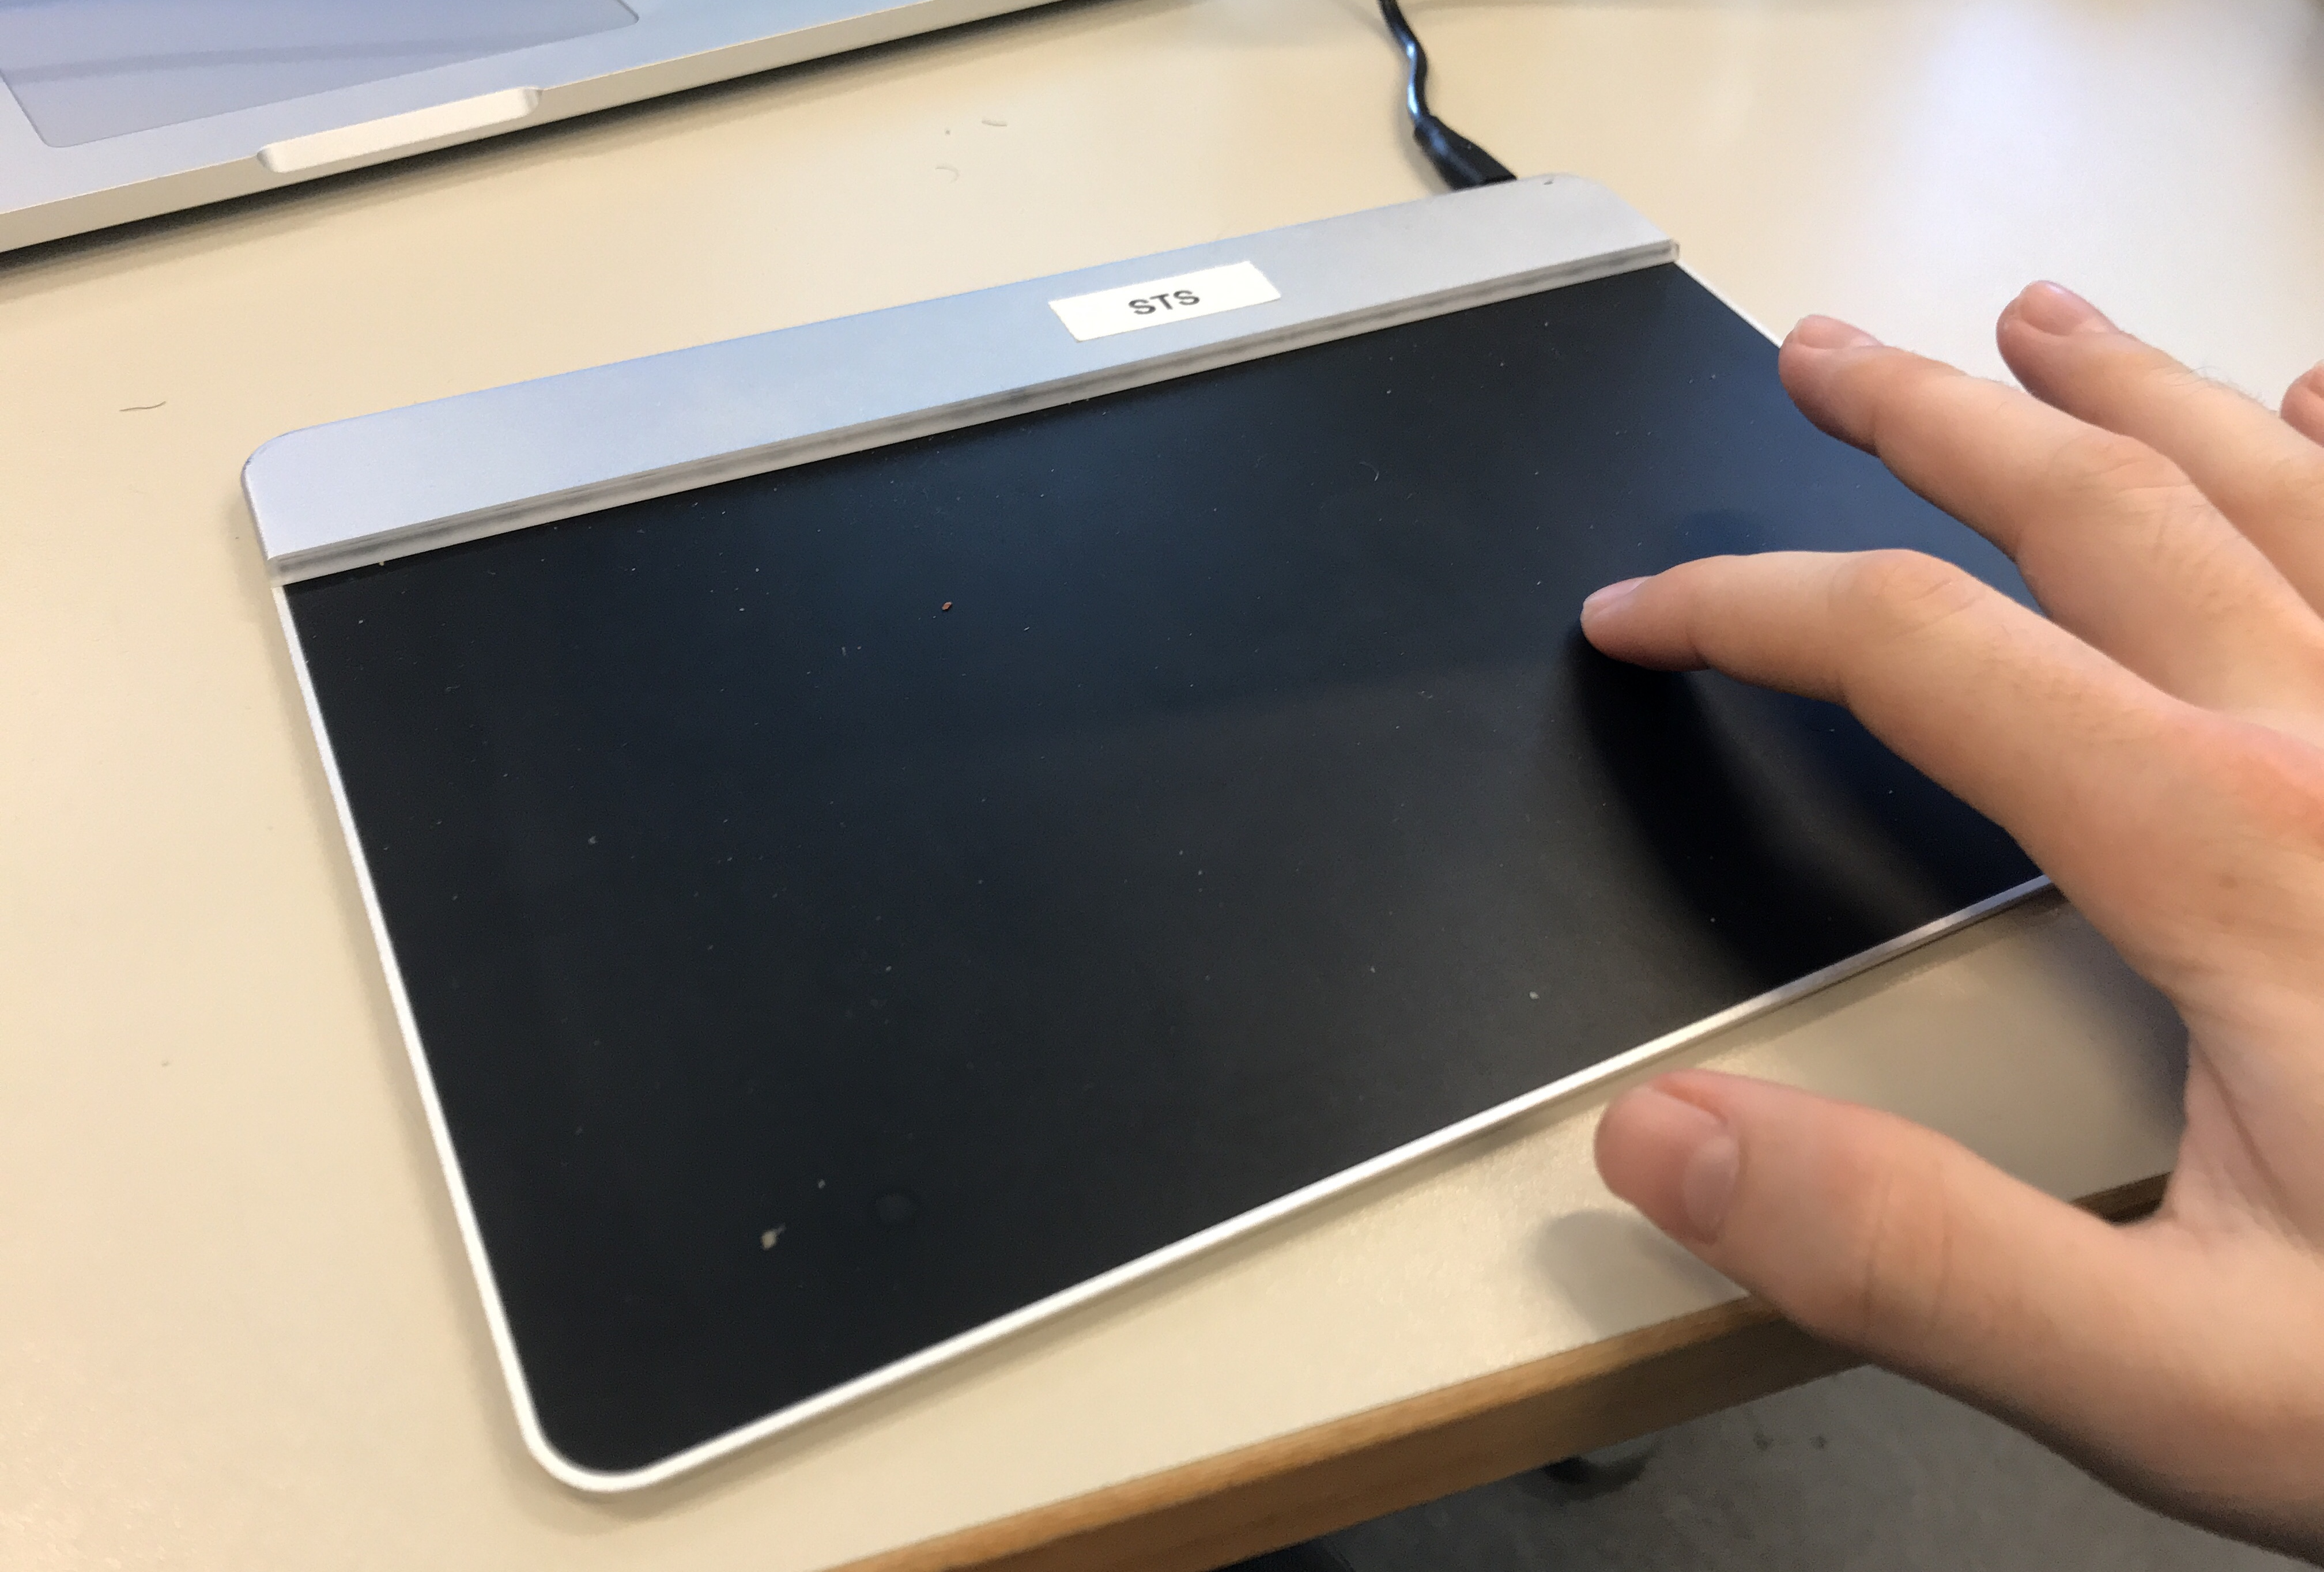
\includegraphics[width=1.0\columnwidth]{IMG_0637.jpg}}
\caption{\label{fig:sensel}{\it The Sensel Morph: an expressive touch sensitive controller used for controlling the real-time elasto-plastic bowed string implementation.}}
\end{figure}

\subsection{Interaction}
The first finger the Sensel registers is linked to the following parameters: the normal force of the bow $f_\text{N}$ (finger pressure), the bowing velocity $v_\text{B}$ (vertical finger velocity) and bowing position $x_\text{B}$ (horizontal finger position). The parameters are limited by the following conditions: $0 \leq f_\text{N} \leq 10$, $-0.3 \leq v_\text{B} \leq 0.3$ and $0<x_\text{B}<L$. The second finger acts as a stopping finger on the string. As done in \cite{Willemsen2019}, for a string stopped at location $x_\text{f}\in[0,L]$ and $l_\text{f}=\text{floor}(x_\text{f}/h)$ we use
\begin{equation}
u_l^n = 
    \begin{cases}
        \hfil 0, & l = l_\text{f} - 1 \vee l = l_\text{f}\\
        \hfil (1-\alpha_\text{f}^\epsilon) u_l^n, & l = l_\text{f} + 1\\
        \hfil u_l^n, & \text{otherwise}
    \end{cases}
\end{equation}
where $\alpha_\text{f} = x_\text{f} / h - l_\text{f}$ and $\epsilon = 7$ is a heuristic value that has been found to most linearly alter pitch between grid points. 

\begin{figure}[ht]
\centerline{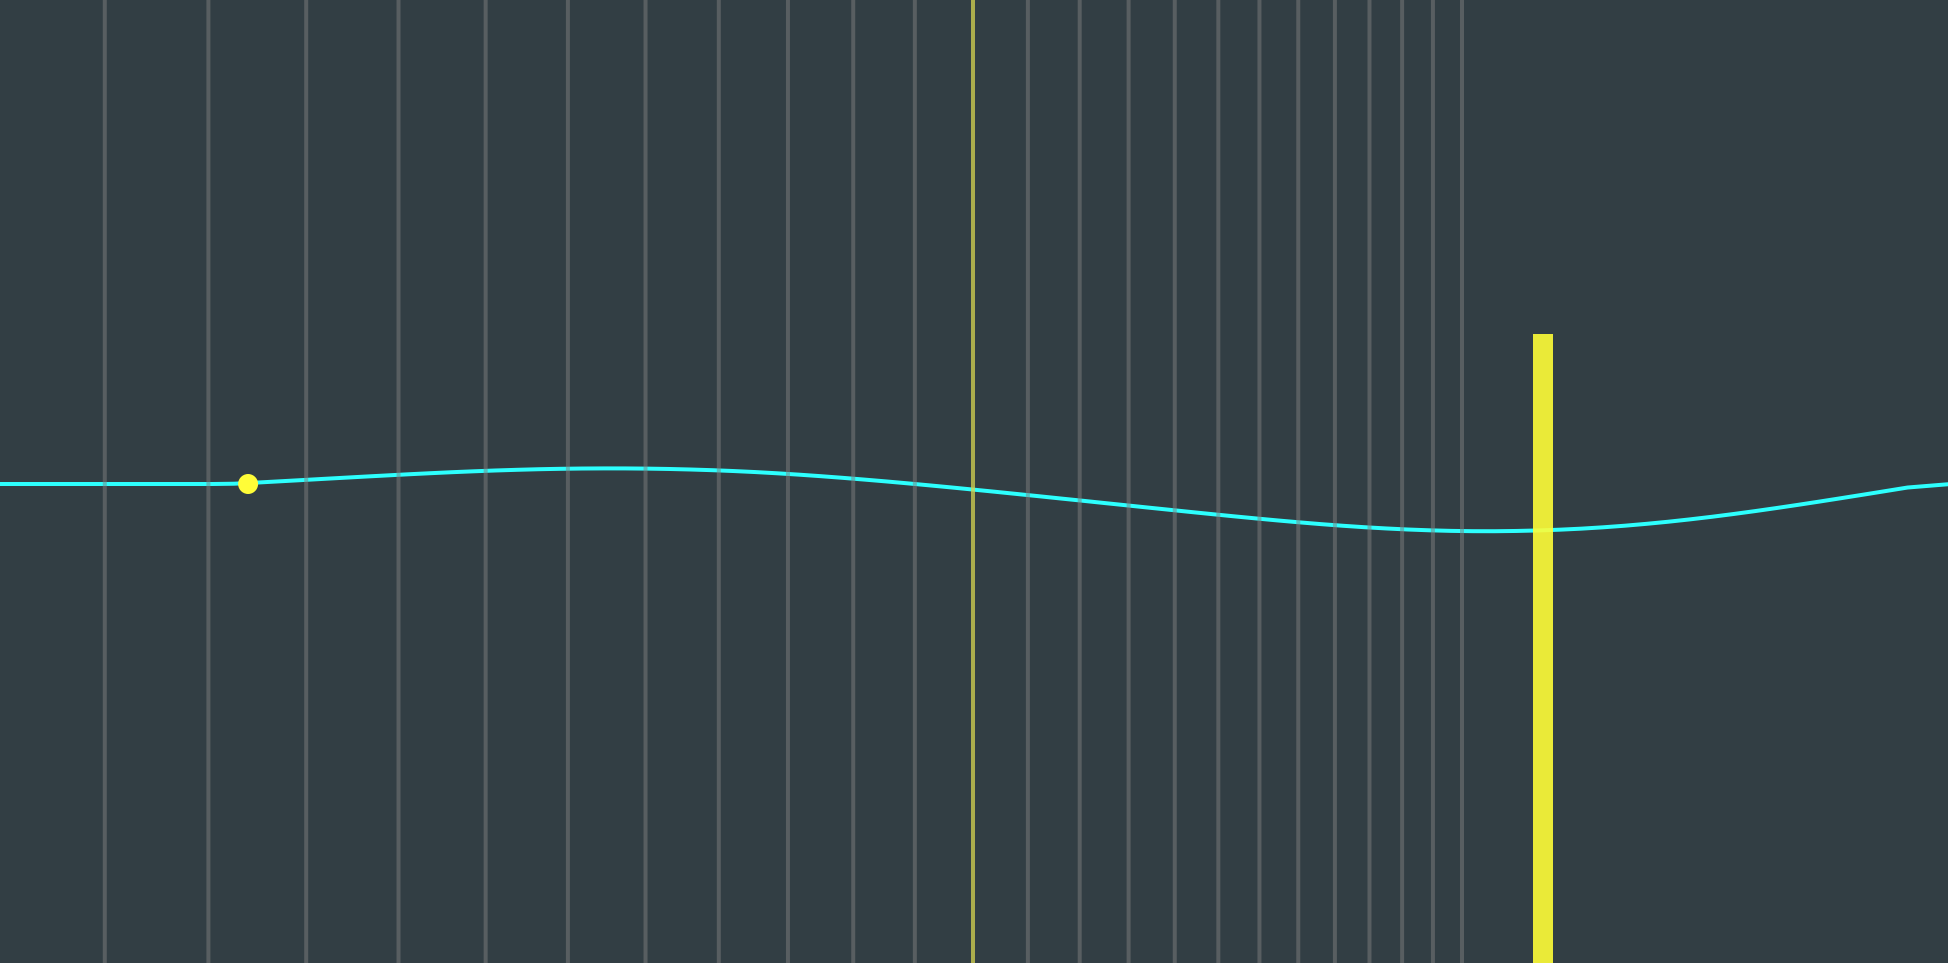
\includegraphics[width=1.0\columnwidth]{JUCEapp.png}}
\caption{\label{fig:application}{\it The elasto-plastic bowed string application. The bow is shown as a yellow rectangle, moves on interaction and its opacity depends on the finger force. The state $\mathbf{u}^n$ is visualised using the cyan curve and stopping-finger position is shown as a yellow circle. The grey lines show the `frets' corresponding to semi-tones as a visual reference for the stopping position and do not influence the model.}}
\end{figure}

\subsection{System Architecture}\label{sec:systemArch}
Implementation of the scheme shown in \eqref{eq:FDS} starts by expanding the operators shown in \eqref{eq:approximations} and solving for the state at the next sample $\mathbf{u}^{n+1}$ where $\mathbf{u}$ is a vector containing the values for all grid points $l\in[0,...,N]$.

An overview of the system architecture can be found in Figure \ref{fig:systemArch}. The three main components of the application are the Sensel controlling the application, the violin string class that performs the simulation and the main application class that moderates between these and the auditory and visual outputs. The black arrows indicate instructions that one of these components can give to another and the hollow arrows indicate data flows. Moreover, the arrows are accompanied by coloured boxes, depicting what thread the instruction or data flow is associated with and at what rate this runs. 

The graphics thread has the lowest priority, is denoted by the green boxes and runs at 15 Hz. The redraw instruction merely retrieves the current string state $\mathbf{u}^n$ and bow and finger position and visualises this as shown in Figure \ref{fig:application}.

The thread checking and receiving data from the Sensel runs at 150 Hz and is denoted by the blue boxes. The parameters that the user interacts with (bowing force, velocity and position) are also updated at this rate.

The highest priority thread is the audio thread denoted by the orange boxes and runs at 44,100 Hz. The violin string class gets updated at this rate and performs operations in the order shown in Algorithm \ref{alg:calcOrder}.
% following order:
% \begin{enumerate}
%     \item Calculate $f(v^n, z^n)$ in \eqref{eq:discForceFunction} using the values for $v^n$ and $z^n$ obtained using NR \eqref{eq:NRit}. 
%     \item Calculate $\mathbf{u}^{n+1}$ using the calculated force function.
%     \item Update the states: switch the (C++) pointer from the vector containing the current values of $\mathbf{u}$ to $\mathbf{u}^{n-1}$ and do the same for $\mathbf{u}^{n+1}$ and $\mathbf{u}$. 
% \end{enumerate}

\begin{figure}[ht]
\centerline{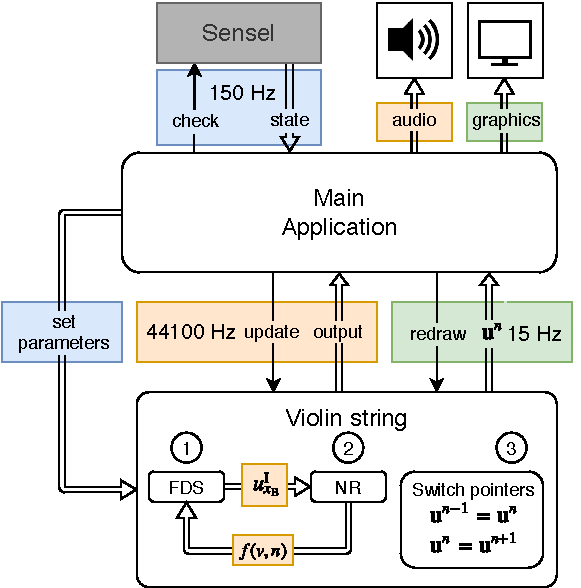
\includegraphics[width=1.0\columnwidth]{systemArchitecture.pdf}}
\caption{\label{fig:systemArch}{\it The system architecture. See Section \ref{sec:systemArch} for a thorough explanation.}}
\end{figure}

\begin{algorithm}[h]
\setstretch{1.25}
\fbox{\parbox{0.9\linewidth}{
 \For{t = 1:lengthSound}{
 calculate computable part $b^n$ (Eq. \eqref{eq:bn})\\
 $\epsilon = 1$\\
 $i = 0$\\
  \While{$\epsilon <$ tol $\wedge\ i < 50 \wedge f_\text{C} > 0$}{
    calculate..
    \vspace{0.15cm}
    \\
\begin{minipage}[c]{0.3\linewidth}
1. $z_\text{ss}(v_{(i)}^n)$ \\
2. $\alpha(v_{(i)}^n,z_{(i)}^n)$ \\
3. $r(v^n_{(i)}, z^n_{(i)})$ \\
4. $g_1$, $g_2$
\end{minipage} 
\begin{minipage}[c]{0.6\linewidth}
(Eq. \eqref{eq:zss} in discrete-time)\\
    (Eq. \eqref{eq:adhesionMap} in discrete-time)\\
    (Eq. \eqref{eq:r})\\
    (Eqs. \eqref{eq:newtonFunction} and \eqref{eq:g2})
\end{minipage}
\vspace{0.01cm}
\\
    5.--9. Compute derivatives of 1.--4. in the same order. \\
    10. Perform vector NR to obtain $v_{(i+1)}^n$ and $z_{(i+1)}^n$\\
    11. Calculate $\epsilon$: $\epsilon = \norm{
    \begin{bmatrix}
    v_{(i+1)}^n\\
    z_{(i+1)}^n
    \end{bmatrix} -
    \begin{bmatrix}
    v_{(i)}^n\\
    z_{(i)}^n
    \end{bmatrix}}$\\
    12. Increment $i$: $i = i + 1$
  }
  Repeat 1.--3. using the values for $v^n$ and $z^n$ from the NR iteration.
  \vspace{0.15cm}
  \\
  \begin{minipage}[c]{0.4\linewidth}
Calculate $f(v^n,z^n)$\\
Calculate $\mathbf{u}^{n+1}$
\end{minipage} 
\begin{minipage}[c]{0.5\linewidth}
(Eq. \eqref{eq:discForceFunction})\\
(Eq. \eqref{eq:FDS} expanded) 
\end{minipage}
  \vspace{0.15cm}
 \\
$\mathbf{u}^{n-1} = \mathbf{u}^n$\\
$\mathbf{u}^{n} = \mathbf{u}^{n+1}$
 }
 }}
 \vspace{0.12cm}
 \caption{Pseudocode showing the order of calculations.\label{alg:calcOrder}}
\end{algorithm}

\section{Results and Discussion}\label{sec:results}

Figure \ref{fig:output44100} shows the outputs waveforms with $f_\text{s} =$ 44,100 Hz and $f_0 = 440$ Hz at different points along the string. The bowing parameters are $f_\text{N} =$ 5 N and $v_\text{B} =$ 0.1 m/s. The figure shows the traditional Helmholtz motion, which is the characteristic motion of a bowed string.

\begin{figure}[h]
  \centering
  \begin{tikzpicture}[->,node distance=3cm,
    thick,main node/.style={circle,draw}]

    \node[anchor=south west,inner sep=0] (image) at (0,0) {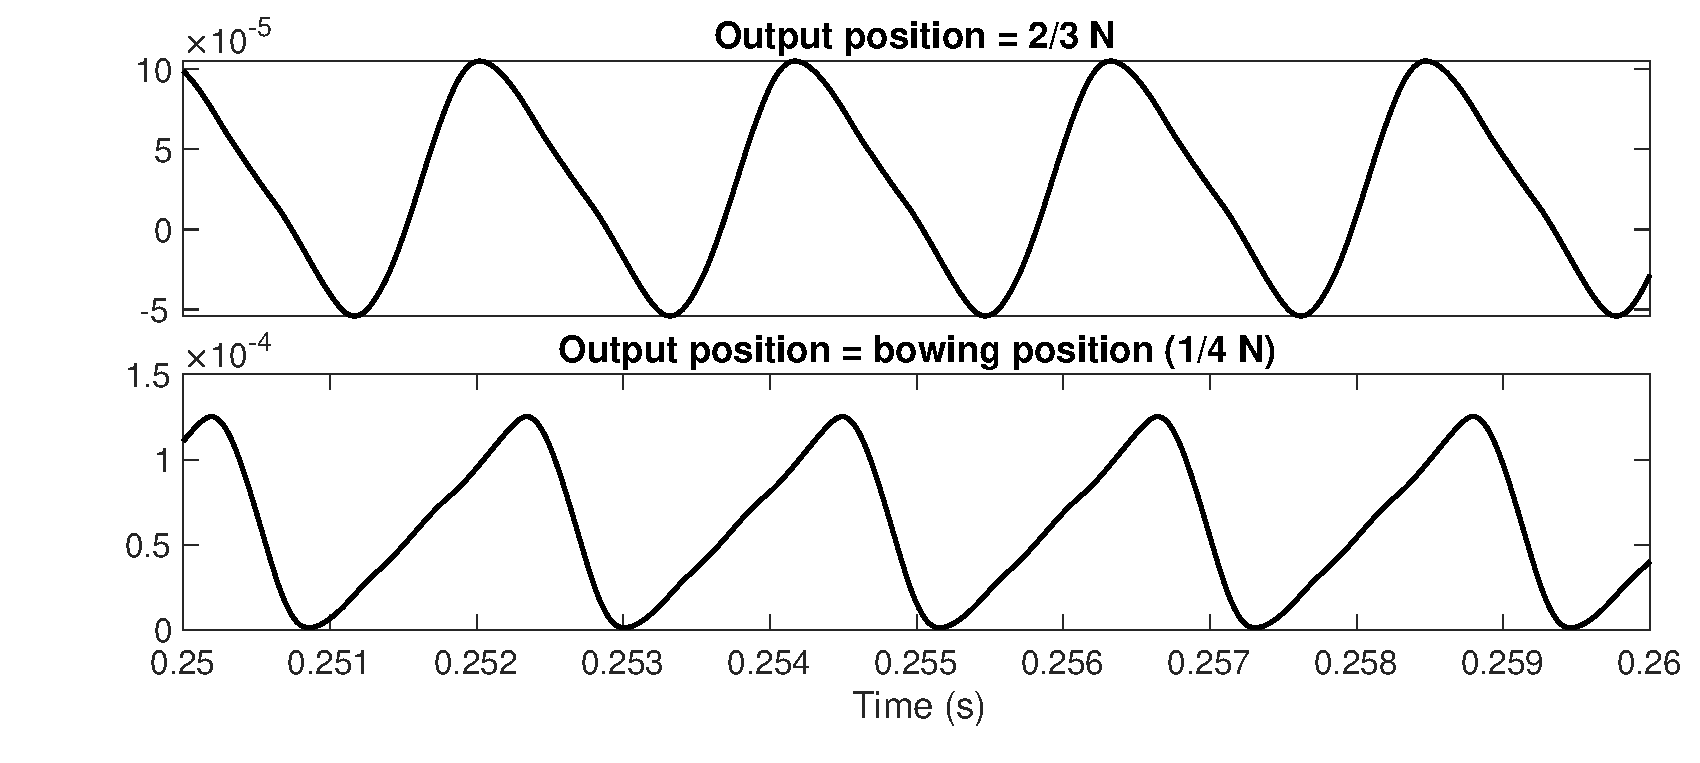
\includegraphics[width=1\columnwidth]{newPaperWaveform.eps}};
    \node (A) at (0.3, 2.8) {a)};
    \node (B) at (0.3, 1.2) {b)};
  \end{tikzpicture}
  \caption{\it Output waveforms of the simulation at different positions along the string where $N$ denotes the number of points of the string ($f_0 =$ 440 Hz, $f_\text{s} =$ 44,100 Hz, $f_\text{N} =$ 5 N and $v_\text{B} =$ 0.1 m/s). \label{fig:output44100}}
\end{figure}

To test whether the implementation exhibits a hysteresis loop, the force vs. relative velocity plane was visualised. In Figure \ref{fig:hysteresis}, this plot can be found for which $f_0 =$ 440 Hz and $f_\text{s} =$ 44,100 Hz have been used. The figure shows values for 500 samples around $t = 0.5f_\text{s}$. As can be seen from the figure, the hysteresis loop is achieved and is similar to the one observed in \cite{Smith2000}. The group of values around $v=0$ are due to the sticking behaviour, and the others (the loop on the left) to the slipping behaviour.

\begin{figure}[h]
  \centering
  \begin{tikzpicture}[->,node distance=3cm,
    thick,main node/.style={circle,draw}]

    \node[anchor=south west,inner sep=0] (image) at (0,0) {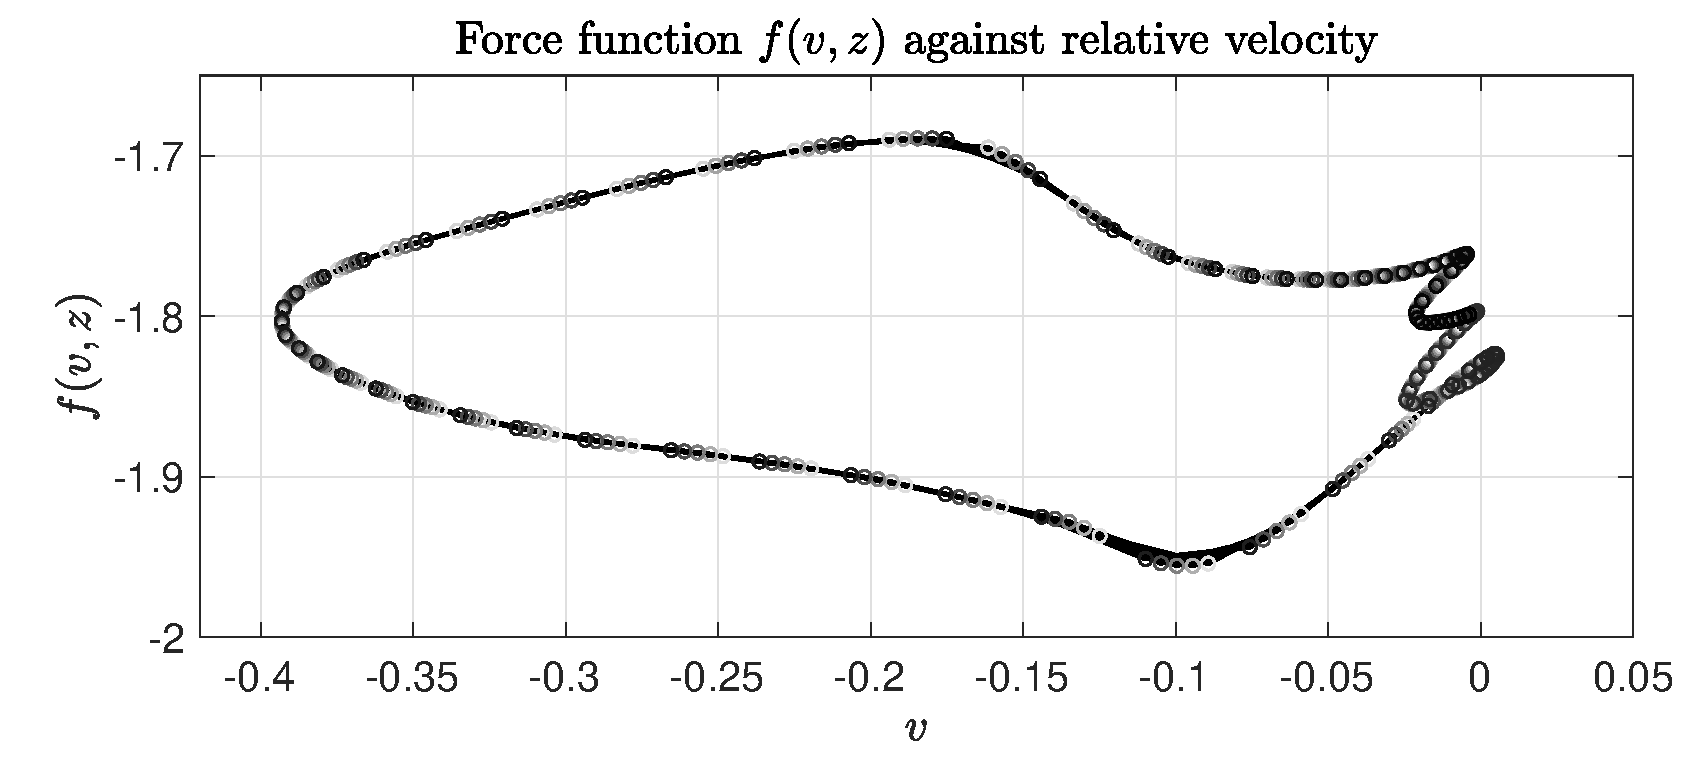
\includegraphics[width=1\columnwidth]{hysteresis3.eps}};
    % \filldraw[black] (arr2B) (2,2) circle (1pt) node[anchor=center](topZ){};
    % \filldraw[black] (arr2E) (3,1.5) circle (1pt) node[anchor=center](topZ){};
    % (arr2B) edge[bend right] node [arrow] {} (arr2E);
    
  \node (arr1B) at (3.8, 3.15) {};
  \node (arr1E) at (5.7, 2.65) {};
  \node (arr2B) at (6.8, 1.2) {};
  \node (arr2E) at (5, 1) {};
  \node (arr3B) at (1.4, 1.7) {};
  \node (arr3E) at (1.5, 2.6) {};
  \path[every node/.style={font=\sffamily\small}]

    (arr1B) edge[bend left = 30] node [left] {} (arr1E)
    (arr2B) edge[bend left = 35] node [left] {} (arr2E)
    (arr3B) edge[bend left = 60] node [left] {} (arr3E);
    % \begin{scope}[x={(image.south east)},y={(image.north west)}]
    %     \draw[red,ultra thick,rounded corners] (0.62,0.65) rectangle (0.78,0.75);
    % \end{scope}
  \end{tikzpicture}
  \caption{\it Hysteresis loop showing 500 values. The values around $v=0$ are due to sticking behaviour and the loop on the left is due to slipping behaviour. \label{fig:hysteresis}}
\end{figure}

Empirical investigation on the behaviour of the model showed that, for low bow forces (around 0.001 N), where a real bowed string shows a so-called multiple slipping, we encounter instability at $f_\text{s} =$ 44,100 Hz \SWcomment[as a result of the NR iteration not being able to converge.]{}. Using higher sample rates resolves this issue. At higher forces, the NR converges after ca. 1-5 iterations.

For testing the speed of the algorithm, a MacBook Pro with a 2.2 GHz Intel Core i7 processor was used. The algorithm was tested using different frequencies according to the violin tuning of \SWcomment[empty strings]: $f_0 = 196.0$ (G3), $293.66$ (D4), $440.0$ (A4) and $659.26$ (E5) Hz corresponding to $N = 60$, $73$, $52$, and $36$ grid points respectively. The results can be seen in Table \ref{tab:results}. When the total number of strings is smaller than 4, always the lowest frequency strings are used.
%This behaviour will require further simulations to be completely understood.
% \begin{table}[h]
%   \caption{{\it Analysis of the amount of iterations for strings with different fundamental frequencies ($f_0$) tested at different sample rates ($f_\text{s}$) for 2 seconds of simulation. The average values are given together with the maximum number of iterations observed. When the capping is used, a percentage is shown denoting the percentage of samples where this capping was used.}}
% 	\centering
%   \begin{tabular}{|c|c|c|c|c|c|c|}\hline
   
%     \multirow{ 2}{*}{\diagbox{$f_0$}{$f_\text{s}$}} & \multicolumn{2}{c|}{44,100}& \multicolumn{2}{c|}{441,000}& \multicolumn{2}{c|}{882,000}\\
%     \cline{2-7}
%     & avg& max &avg &max & avg & max\\
%     \hline
%     196.00 & 3.35 & 1.18 \% & 2.50& 0.03\% & 2.33 & 7 \\
%     293.66 & 3.14 & 0.64\% & 2.37 & 0.007\% & 2.11 & 6\\
%     440.00 & 2.99 & 0.27\% & 2.57 & 10& 2.15 & 6\\
%     659.26 & 3.29 & 10 & 2.73 & 8 & 2.54 & 6 \\
%     \hline
%  \end{tabular}
% 	%
%   \label{tab:results}
% \end{table}

\begin{table}[h]
  \caption{{\it CPU usage for different amounts of strings. The values are averages over a 10 s period both for the enabled and disabled graphics thread. All strings are bowed simultaneously (polyphonically).}}
	\centering
  \begin{tabular}{|c|c|c|}\hline
   
    Amount of strings & Graphics (\%) & No graphics (\%)\\
    \hline
    1 & 42.8 / 50.5 & 7.0 / 14.5\\
    2 &  & \\
    3 &  & \\
    4 &  & \\
    \hline
 \end{tabular}
	%
  \label{tab:results}
\end{table}

From Table \ref{tab:results} it can be observed that for one string, the CPU usage is $<5\%$ with the graphics thread disabled. This is a great result, given the fact that both the bow and the string model are computationally complex. A single string (but also more) could thus safely be used as an audio plugin in parallel to others without the user having to worry about auditory dropouts. Furthermore, it can be observed that the differences in CPU usage decrease as the number of strings increases. This can be explained by the fact that the number of points for higher strings are less than that of lower strings and thus need less computational power.

\section{Conclusions}\label{sec:conclusion}
In this paper, we presented an implementation of an elasto-plastic friction model with applications to a  bow exciting a string, discretised using a finite-difference approach. 

With a single string we are able to keep the CPU usage down to $<5\%$ making for an efficient implementation that could be used in parallel with other virtual instruments or plugins.

Future work includes parameter design and including an instrument body for more realistic sounding results, as well as listening tests to verify the perceivable differences between simpler friction models versus the elasto-plastic model.



\section{Acknowledgments}
Many thanks to the anonymous reviewers for giving their valuable input. This work is supported by NordForsk's Nordic
University Hub Nordic Sound and Music Computing Network
NordicSMC, project number 86892.

%\newpage
%\nocite{*}
\begin{footnotesize}
\bibliographystyle{IEEEbib}
\bibliography{DAFx19_tmpl} 
\end{footnotesize}
% requires file DAFx19_tmpl.bib

% \section{Appendix: Interpolation and Spreading Operators}
% \label{app:interpol}
% In this section, the interpolator and spreading operator introduced in Section \ref{sec:discretisation} will be explained. More information can be found in \cite{Bilbao2009}.

% The interpolator $I$ and spreading operator $J$ are vectors the size of $\mathbf{u}$ described in Section \ref{sec:systemArch}. The simplest way to select a grid point $l_\text{B}$ from bowing position $x_\text{B}$ on a discrete string is $l_\text{B} = \text{floor}(x_\text{B}/h)$. Applied to a gridfunction $u_l$ yields
% \begin{equation}
%     I_0(x_\text{B})u_l = u_{l_\text{B}}.
% \end{equation}
% More accurate would be to use linear interpolation 
% \begin{equation}\label{eq:linearInterpolation}
%      I_1(x_\text{B})u_l =
%       (1-\alpha_\text{B})u_{l_\text{B}}+ \alpha_\text{B}u_{l_\text{B}+1}
% \end{equation}
% where $\alpha_\text{B} = x_\text{B}/h - l_\text{B}$ is the fractional remainder of the flooring operation. Even more accurate would be to use cubic interpolation:
% % \begin{equation}\label{eq:cubicInterpolation}
% % \begin{aligned}
% %      I_3(x_\text{B})u_{l_\text{B}} =&  \frac{\alpha_\text{B}(\alpha_\text{B}-1)(\alpha_\text{B} - 2)}{-6}u_{l_\text{B}-1}+\\
% %      &\frac{(\alpha_\text{B}-1)(\alpha_\text{B}+1)(\alpha_\text{B}-2)}{2}u_{l_\text{B}}+  \frac{\alpha_\text{B}(\alpha_\text{B}+1)(\alpha_\text{B} - 2)}{-2}u_{l_\text{B}+1} \\
% %      &+ \frac{\alpha_\text{B}(\alpha_\text{B}+1)(\alpha_\text{B} - 1)}{6}u_{l_\text{B}+2}
% %      \end{aligned}
% % \end{equation}
% \begin{equation}
% I_3(x_\text{B}) =
%      \begin{cases}
%     \hfil 0, & l < l_{\text{B}} - 1\\
%     \hfil \alpha_\text{B}(\alpha_\text{B}-1)(\alpha_\text{B} - 2)/{-6}, & l = l_{\text{B}} - 1\\
%     \hfil (\alpha_\text{B}-1)(\alpha_\text{B}+1)(\alpha_\text{B}-2)/2, & l = l_{\text{B}}\\
%     \hfil \alpha_\text{B}(\alpha_\text{B}+1)(\alpha_\text{B} - 2)/{-2}, & l = l_{\text{B}} + 1\\
%     \hfil \alpha_\text{B}(\alpha_\text{B}+1)(\alpha_\text{B} - 1)/6, & l = l_{\text{B}} +2,\\
%     \hfil 0, & l > l_\text{B} + 2
%     \end{cases}
%     \end{equation}
% Similarly, the spreading operator $J$ can be defined as linear:
% \begin{equation}\label{eq:linearSpreading}
%      J_1(x_\text{B}) = \frac{1}{h}
%      \begin{cases}
%     \hfil 0, & l < l_{\text{B}}\\
%     \hfil (1-\alpha_\text{B}), & l = l_{\text{B}}\\
%     \hfil \alpha_\text{B}, & l = l_{\text{B}} + 1\\
%     \hfil 0, & l > l_\text{B} + 1
% \end{cases}
% \end{equation}
% or cubic:
% \begin{equation}\label{eq:cubicInterpolation}
%      J_3(x_\text{B}) = \frac{1}{h}
%      \begin{cases}
%     \hfil 0, & l < l_{\text{B}} - 1\\
%     \hfil \alpha_\text{B}(\alpha_\text{B}-1)(\alpha_\text{B} - 2)/{-6}, & l = l_{\text{B}} - 1\\
%     \hfil (\alpha_\text{B}-1)(\alpha_\text{B}+1)(\alpha_\text{B}-2)/2, & l = l_{\text{B}}\\
%     \hfil \alpha_\text{B}(\alpha_\text{B}+1)(\alpha_\text{B} - 2)/{-2}, & l = l_{\text{B}} + 1\\
%     \hfil \alpha_\text{B}(\alpha_\text{B}+1)(\alpha_\text{B} - 1)/6, & l = l_{\text{B}} +2,\\
%     \hfil 0, & l > l_\text{B} + 2
% \end{cases}
% \end{equation}
% Note the scaling with $1/h$.
\end{document}
